\PassOptionsToPackage{unicode=true}{hyperref} % options for packages loaded elsewhere
\PassOptionsToPackage{hyphens}{url}
%
\documentclass[12pt,italian,]{report}
\usepackage{lmodern}
\usepackage{amssymb,amsmath}
\usepackage{ifxetex,ifluatex}
\usepackage{fixltx2e} % provides \textsubscript
\ifnum 0\ifxetex 1\fi\ifluatex 1\fi=0 % if pdftex
  \usepackage[T1]{fontenc}
  \usepackage[utf8]{inputenc}
  \usepackage{textcomp} % provides euro and other symbols
\else % if luatex or xelatex
  \usepackage{unicode-math}
  \defaultfontfeatures{Ligatures=TeX,Scale=MatchLowercase}
\fi
% use upquote if available, for straight quotes in verbatim environments
\IfFileExists{upquote.sty}{\usepackage{upquote}}{}
% use microtype if available
\IfFileExists{microtype.sty}{%
\usepackage[]{microtype}
\UseMicrotypeSet[protrusion]{basicmath} % disable protrusion for tt fonts
}{}
\IfFileExists{parskip.sty}{%
\usepackage{parskip}
}{% else
\setlength{\parindent}{0pt}
\setlength{\parskip}{6pt plus 2pt minus 1pt}
}
\usepackage{hyperref}
\hypersetup{
            pdftitle={Progetto Usabilità e User Experience 2018/2019},
            pdfauthor={Filippo Bartolini; Adamo Fapohunda; Giacomo Leidi; Cristian Castiglione},
            pdfborder={0 0 0},
            breaklinks=true}
\urlstyle{same}  % don't use monospace font for urls
\usepackage{longtable,booktabs}
% Fix footnotes in tables (requires footnote package)
\IfFileExists{footnote.sty}{\usepackage{footnote}\makesavenoteenv{longtable}}{}
\usepackage{graphicx,grffile}
\makeatletter
\def\maxwidth{\ifdim\Gin@nat@width>\linewidth\linewidth\else\Gin@nat@width\fi}
\def\maxheight{\ifdim\Gin@nat@height>\textheight\textheight\else\Gin@nat@height\fi}
\makeatother
% Scale images if necessary, so that they will not overflow the page
% margins by default, and it is still possible to overwrite the defaults
% using explicit options in \includegraphics[width, height, ...]{}
\setkeys{Gin}{width=\maxwidth,height=\maxheight,keepaspectratio}
\setlength{\emergencystretch}{3em}  % prevent overfull lines
\providecommand{\tightlist}{%
  \setlength{\itemsep}{0pt}\setlength{\parskip}{0pt}}
\setcounter{secnumdepth}{0}
% Redefines (sub)paragraphs to behave more like sections
\ifx\paragraph\undefined\else
\let\oldparagraph\paragraph
\renewcommand{\paragraph}[1]{\oldparagraph{#1}\mbox{}}
\fi
\ifx\subparagraph\undefined\else
\let\oldsubparagraph\subparagraph
\renewcommand{\subparagraph}[1]{\oldsubparagraph{#1}\mbox{}}
\fi

% set default figure placement to htbp
\makeatletter
\def\fps@figure{htbp}
\makeatother

\ifnum 0\ifxetex 1\fi\ifluatex 1\fi=0 % if pdftex
  \usepackage[shorthands=off,main=italian]{babel}
\else
  \usepackage{polyglossia}
  \setmainlanguage[]{italian}
\fi

\title{Progetto Usabilità e User Experience 2018/2019\\[0.8em]\large CdLM Informatica - Università di Bologna}
\author{Filippo Bartolini 0000 \\ Adamo Fapohunda 0000\\ Giacomo Leidi 0000 \\ Cristian Castiglione 0000}
\date{}

\begin{document}
\maketitle

{
\setcounter{tocdepth}{2}
\tableofcontents
}
\newpage
\section{Introduzione}\label{introduzione}
Kids Experience è un applicativo web legato al sito madre Kiabi.

Kiabi è un'azienda francese di e-commerce e distribuzione di
abbigliamento pronto moda, facente parte del gruppo Mulliez. Il suo
slogan \emph{``La moda a piccoli prezzi''} si basa su prodotti a prezzi
accessibili per tutta la famiglia.

Kids Experience offre ai clienti la possibilità di personalizzare
autonomamente megliette per bambini e ragazzi, da 3 a 12 anni, ampliando la vasta gamma di prodotti offerti da Kiabi.

Il punto di forza di questa nuova categoria di prodotti è costituito dall'estrema personalizzazione di magliette per bambini offerta all'utente.

\section{Ricerca etnografica}\label{ricerca-etnografica}
È possibile subito osservare come i bisogni che Kids Experience andrà a soddisfare non si trovino nei primi livelli della gerarchia di Maslow, ma si identifichino nel livello intermedio della gerarchia: il livello
di \emph{appartenenza}.

Successivamente si è fatta un'analisi del mercato dell'abbigliamento, analizzando alcuni competitors attraverso dati reperiti online.
Precisamente, come si evince dalla Fig \ref{abbigliamo_generico}, per quanto riguarda il
mercato italiano il maggiore esponente è risultato essere Zara, mentre Kiabi si posiziona al terzo posto.

\begin{figure}[h]
\centering
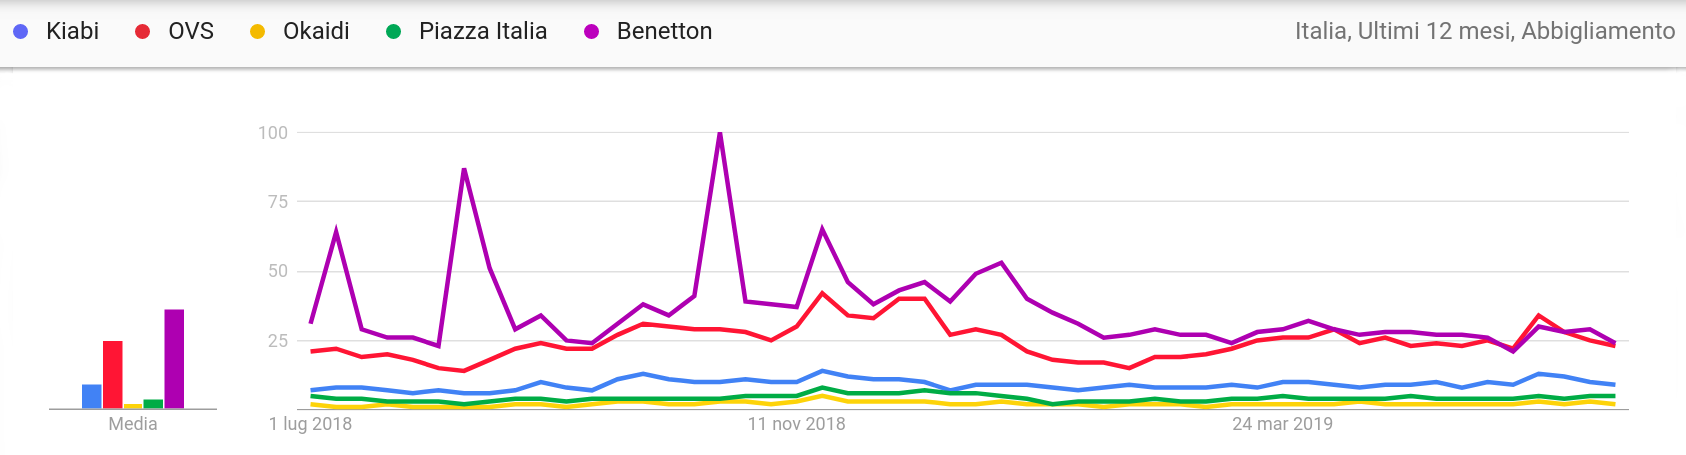
\includegraphics{img/abbigliamento_generico.png}
\caption{Ricerca di mercato - abbigliamento}
\label{abbigliamo_generico}
\end{figure}

Per quanto riguarda il mercato dell'abbigliamento da bambino, Kiabi perde un ulteriore posizione passando dal terzo al quarto posto, come mostrato in Fig. \ref{abbigliamento_bambino}.

\begin{figure}[h]
\centering
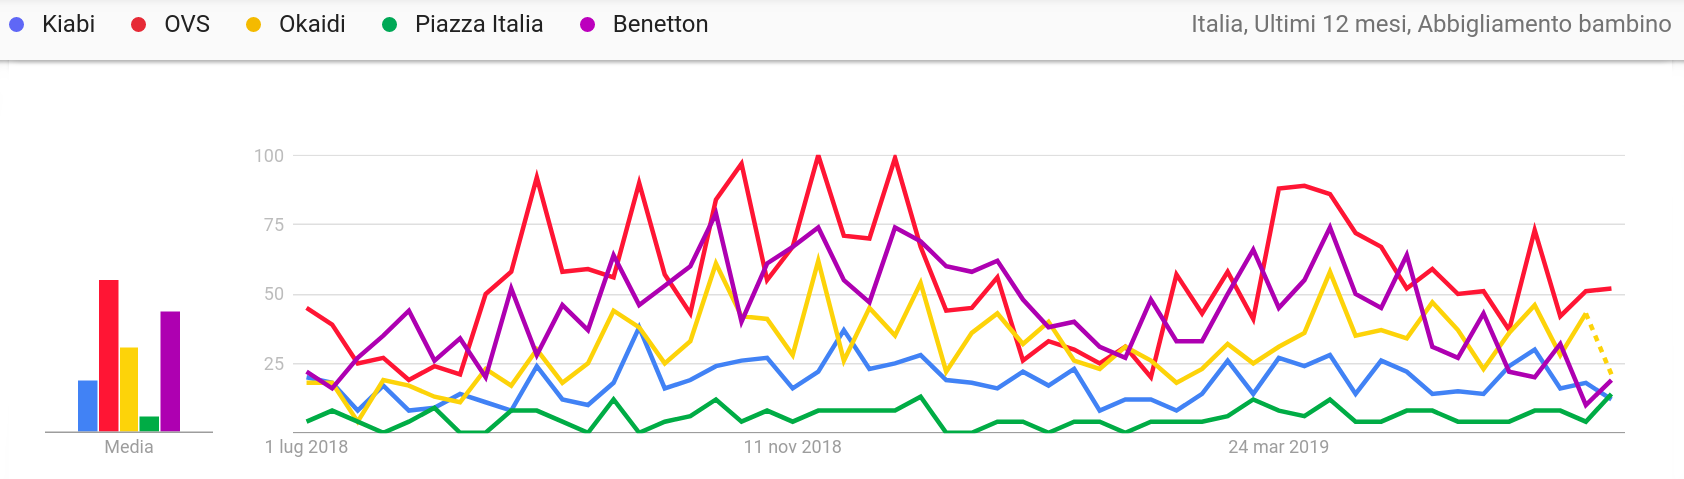
\includegraphics{img/abbigliamento_bambino.png}
\caption{Ricerca di mercato - abbigliamento bambino}
\label{abbigliamento_bambino}
\end{figure}

Dopo un'attenta analisi abbiamo deciso di prendere Kiabi come azienda madre, con l'obiettivo di rilanciarla sul mercato dell'abbigliamento per bambina/o tramite l'aggiunta di nuove features da noi ideate e proposte al Project Manager Mulliez.

L'idea di progettare magliette estremamente perzonalizzabili solo per bambini, nasce dalla semplicità del capo dettati dai minimi vincoli fisici (i.e. taglia) del target. Questo permette di garantire all'utente un'ampia gamma di personalizzazioni senza dover complicare eccessivamente
il processo di manifattura.

\newpage
\section{Blueprint}\label{Blueprint}
Le blueprint sono semplici diagrammi che definiscono l'organizzazione dei contenuti e come le varie componenti interagiscono tra di loro.

Saranno presentate quattro blueprint che mostrano, rispettivamente:

\begin{enumerate}
\def\labelenumi{\arabic{enumi}.}
\tightlist
\item
  Creazione di un nuovo modello
\item
  Organizzazione delle azioni disponibili per un utente loggato
\item
  Organizzazione delle azioni disponibili per un utente non loggato
\end{enumerate}
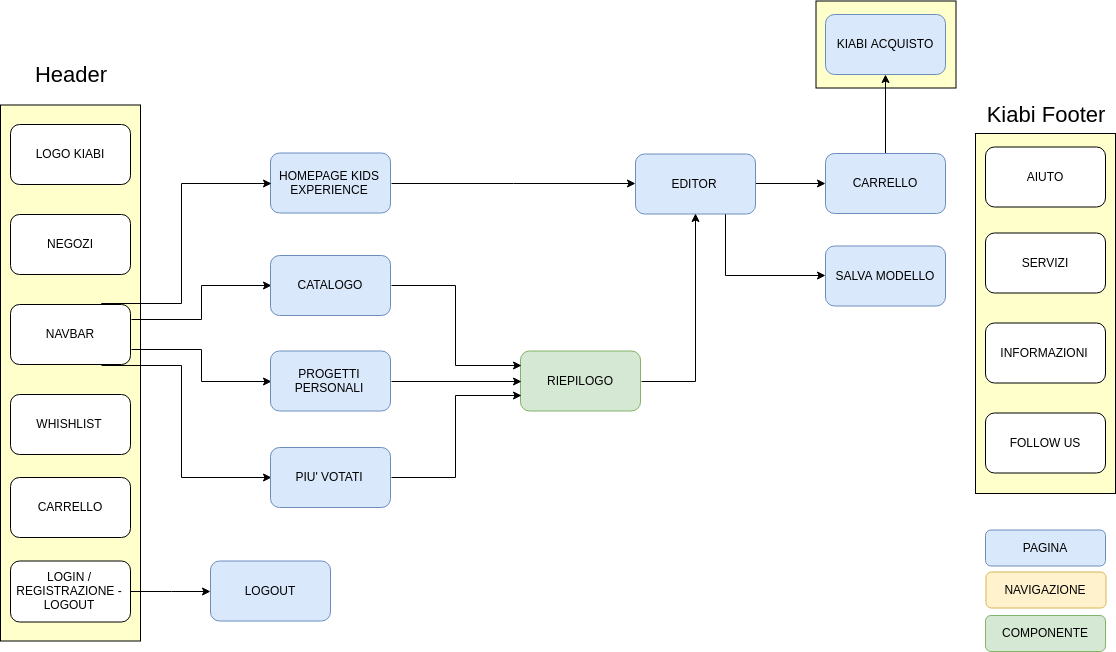
\includegraphics{blueprints/Utente_loggato.png}
\\
\\
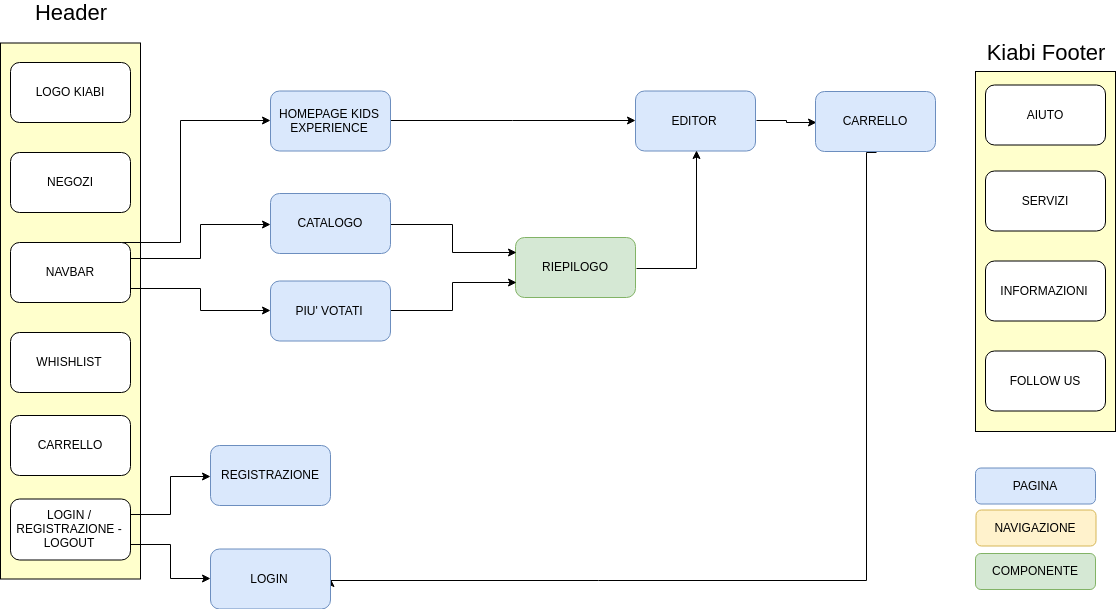
\includegraphics{blueprints/Utente_non_loggato.png}
\\
\\
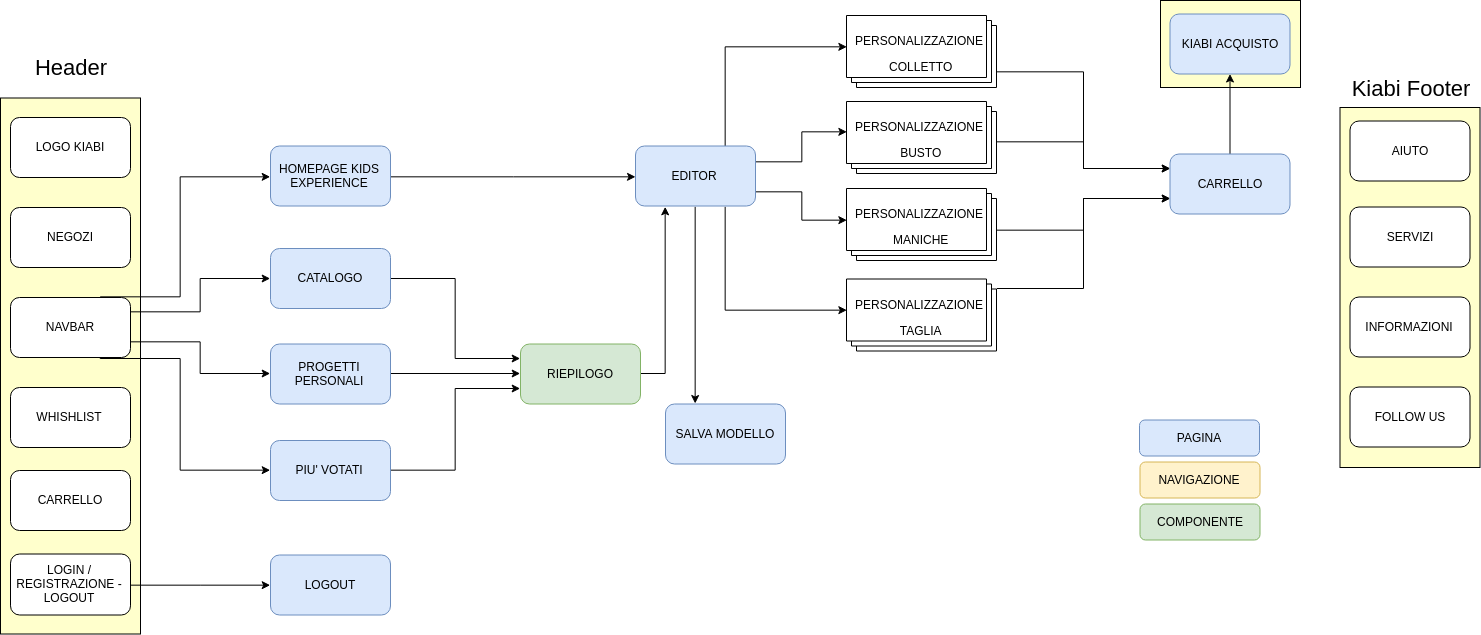
\includegraphics{blueprints/Creazione_modello.png}
\newpage
\section{Wireframes}\label{Wireframes}

\subsection{Home Kiabi}

I wireframe in Fig. \ref{kiabi_home} e Fig \ref{kiabi_home_selection} mostrano la homepage del sito kiabi con l'aggiunta dei collegamenti per raggiungere il sottosito Kids Experience.

\begin{figure}[h]
\centering
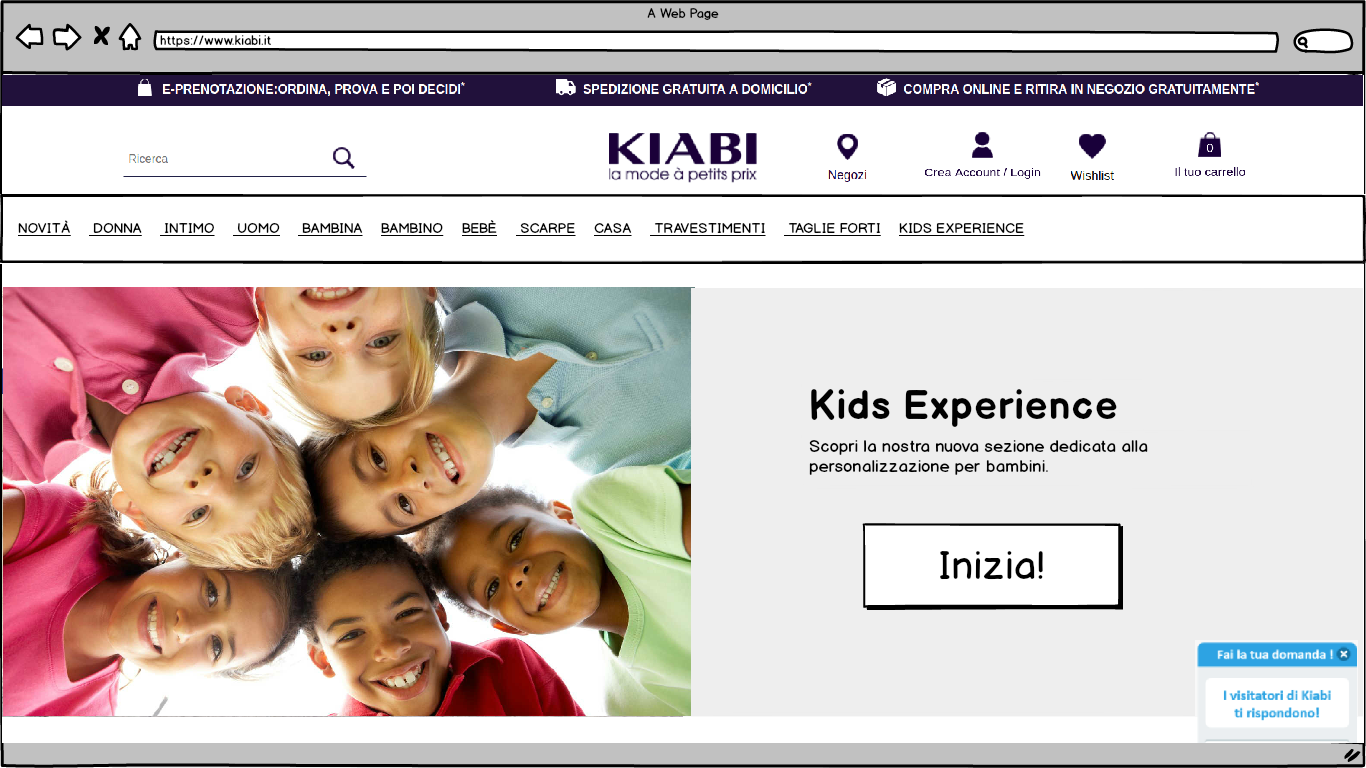
\includegraphics{../../balsamiq/balsamiq_finale/KiabiHome.png}
\caption{Home Kiabi con link a Kids Experience}
\label{kiabi_home}
\end{figure}

\begin{figure}[h]
\centering
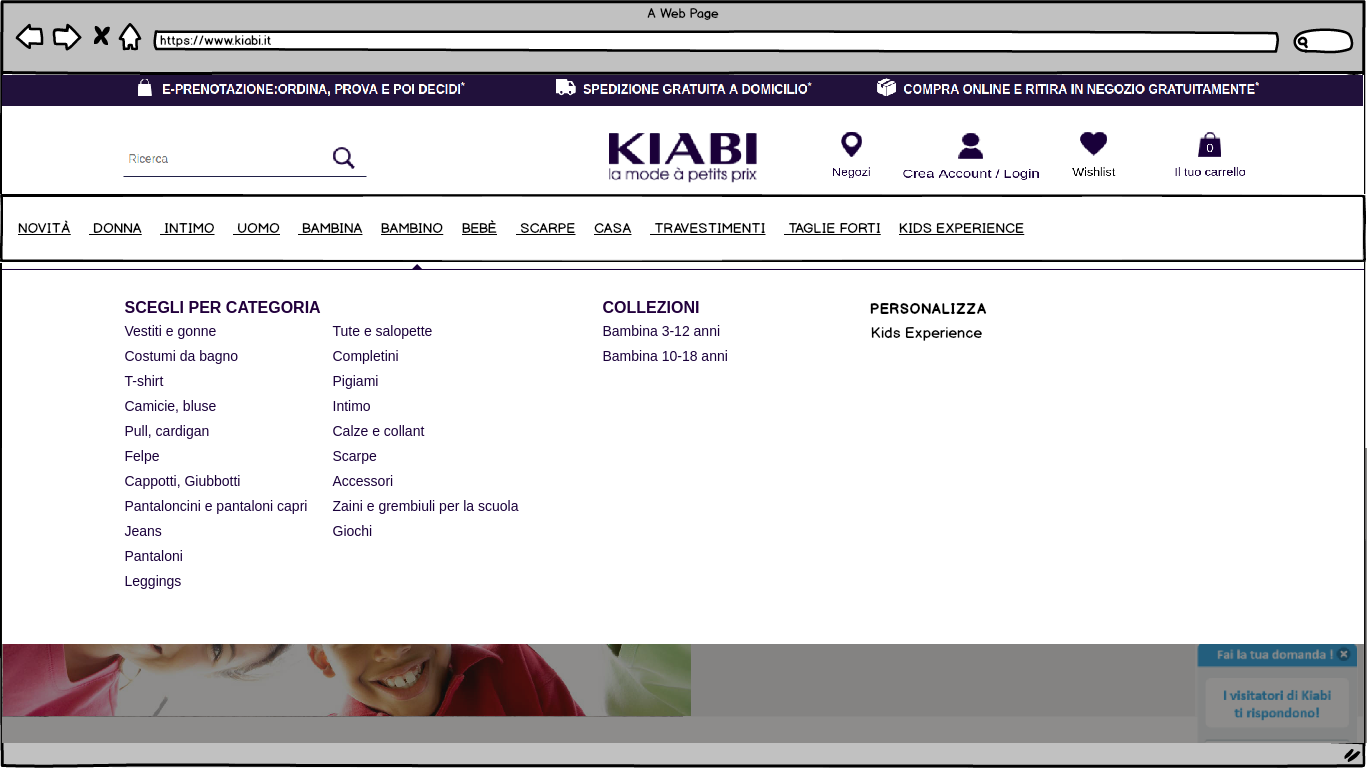
\includegraphics{../../balsamiq/balsamiq_finale/KiabiScelta.png}
\caption{Home Kiabi - Menù bambino/a con link a Kids Experience}
\label{kiabi_home_selection}
\end{figure}

\newpage
\subsection{Home Kids Experience} 

La home è composta da tre elementi: un header, un corpo, e un footer.
\begin{itemize}
\item
L’header rimane fisso in alto quando si scrolla la pagina, in quanto contiene elementi che possono richiedere un accesso veloce durante la visita della pagina. 
A sua volta è diviso in due sezioni. La parte in alto è identica al sito madre. La parte in basso, invece, contiene la navbar che sostituisce quella già presente nel sito kiabi.

\item
Il corpo ricopre due funzioni. 
La prima è quella di fornire un collegamento diretto all'editor corredato da reclame pubblicitaria, molto più visibile del link già presente nella navbar. 
La seconda è quella di fornire un tutorial di base sull'utilizzo dell'editor.

\item Il footer contiene elementi marginali contenenti informazioni sul sito madre kiabi.
\end{itemize}

\begin{figure}[h]
\centering
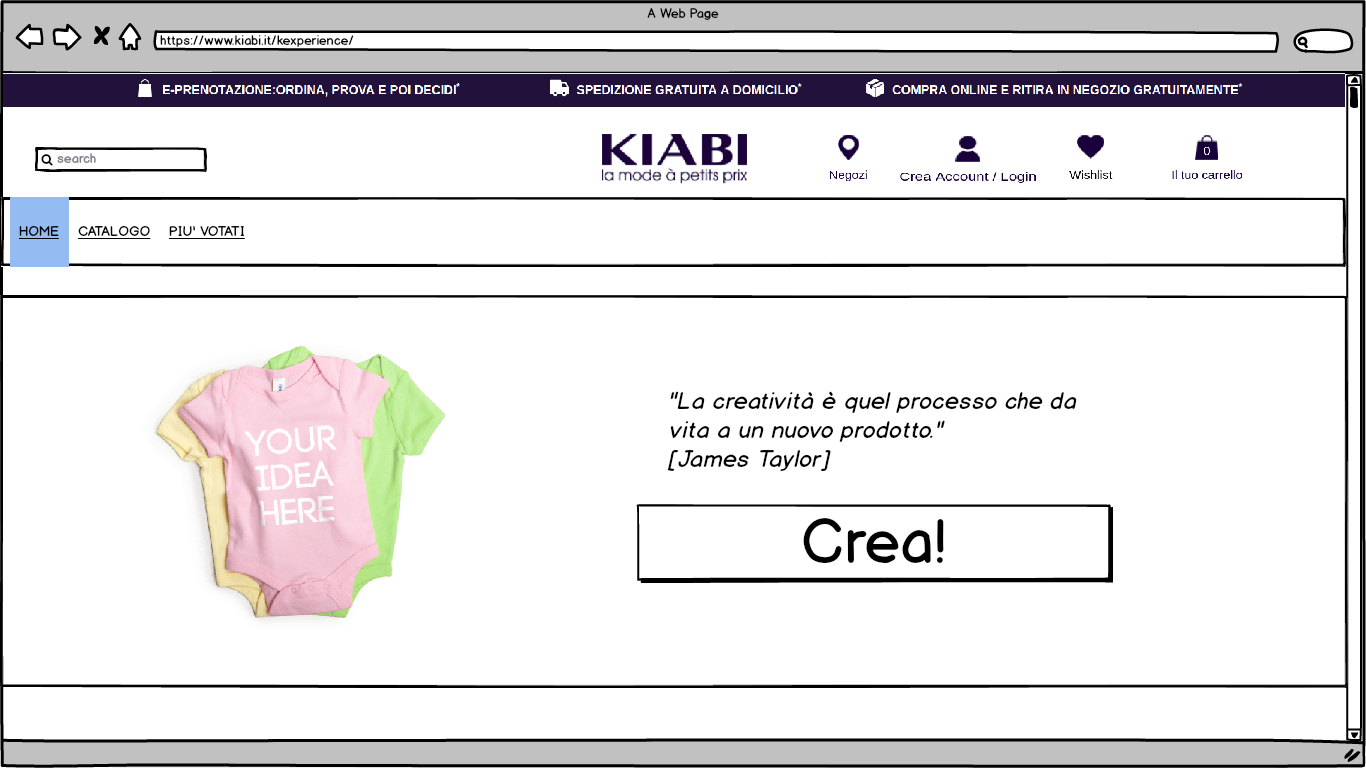
\includegraphics{../../balsamiq/balsamiq_finale/HomeSottositoUtenteEsterno.png}
\caption{Home Kids Experience}
\label{kids_home}
\end{figure}




\subsection{Catalogo} 

La sezione catalogo (Fig. \ref{catalogo}) è facilmente raggiungibile a partire dalla navbar.

\begin{figure}[h]
\centering
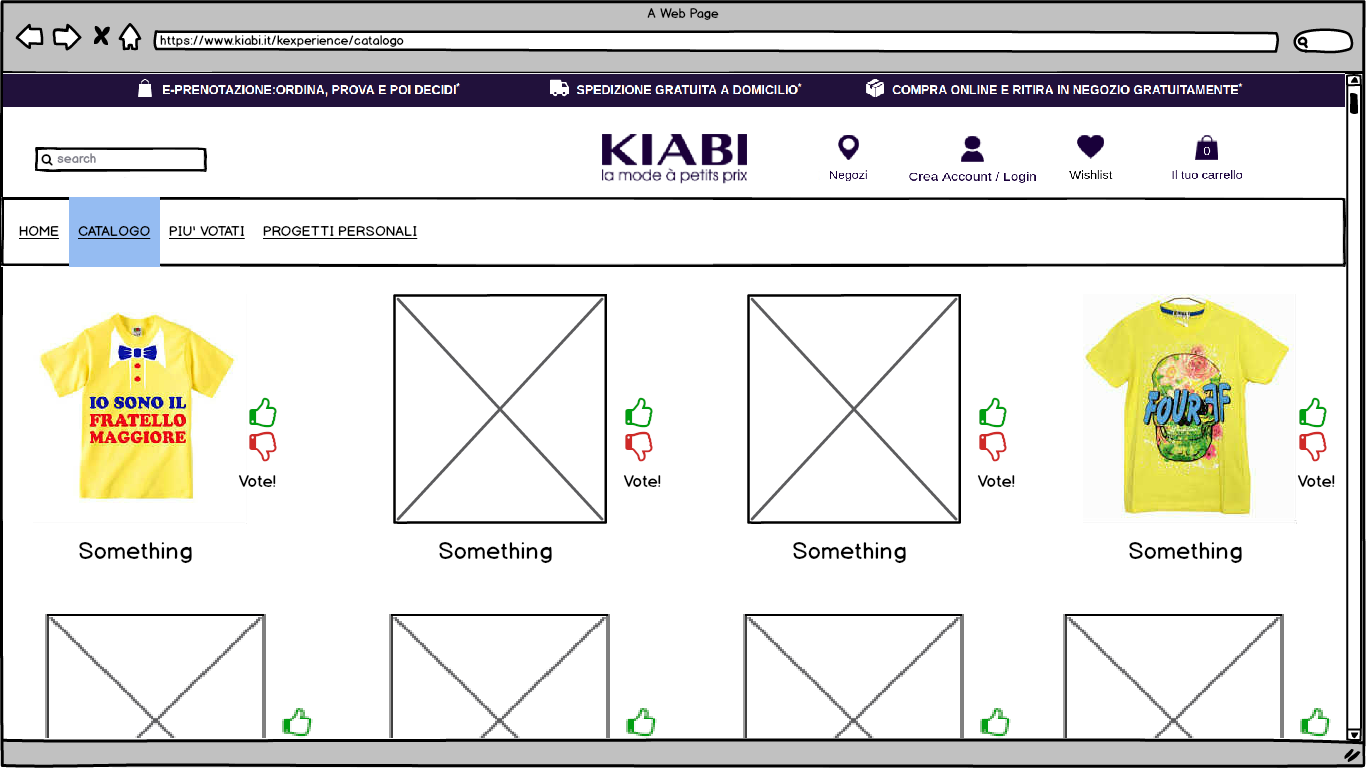
\includegraphics{../../balsamiq/balsamiq_finale/Catalogo.png}
\caption{Sezione Catalogo}
\label{catalogo}
\end{figure}

Questa contiene la lista dei prodotti di Kids Experience ordinati per data di creazione. Tramite la searchbar è possibile effettuare ricerche in linguaggio naturale. È possible cercare per autore, nome, colore e taglia. Aggiungendo attributi come "bottoni colletto" verrà effettuata una query per ricercare in tutti i prodotti che contengono quel tag nella lista di personalizzazioni.

Con un click su una maglietta è possibile visionare i dettagli di questa: la lista delle modifiche, l'autore e il prezzo. Dal modale (Fig. \ref{catalogo_dettagli}) è anche possibile modificare il prodotto entrando nell'editor.

Facendo over con il mouse su una maglietta, compaiono i due tasti di like/dislike più il tasto condividi. Mentre la condivisione è sempre possibile, la funzionalità di votazione tramite like/dislike è disabilitata per l'utente che non ha effettuato il login. In tal caso compare il messaggio mostrato in Fig. \ref{catalogo_non_loggato}.

\begin{figure}[h]
\centering
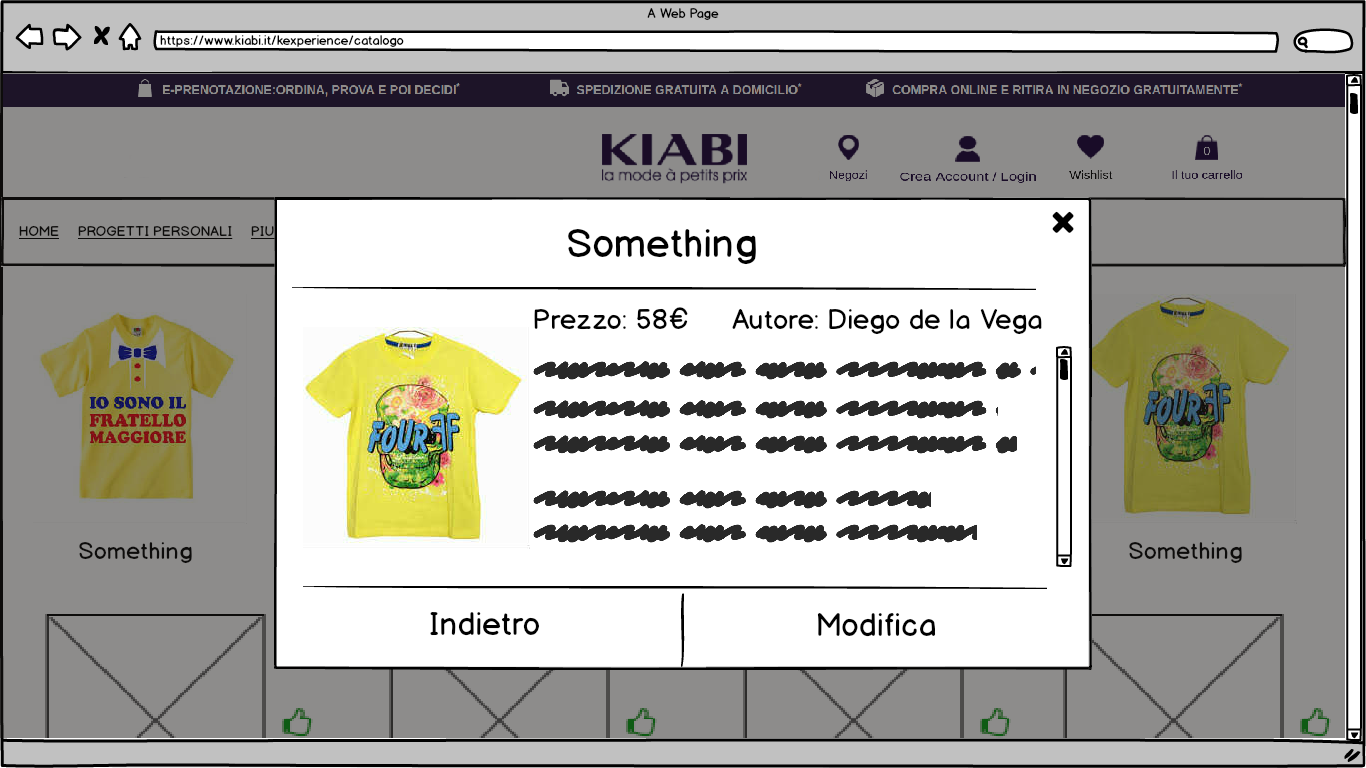
\includegraphics{../../balsamiq/balsamiq_finale/Catalogodetails.png}
\caption{Sezione Catalogo - Dettagli prodotto}
\label{catalogo_dettagli}
\end{figure}

\begin{figure}[h]
\centering
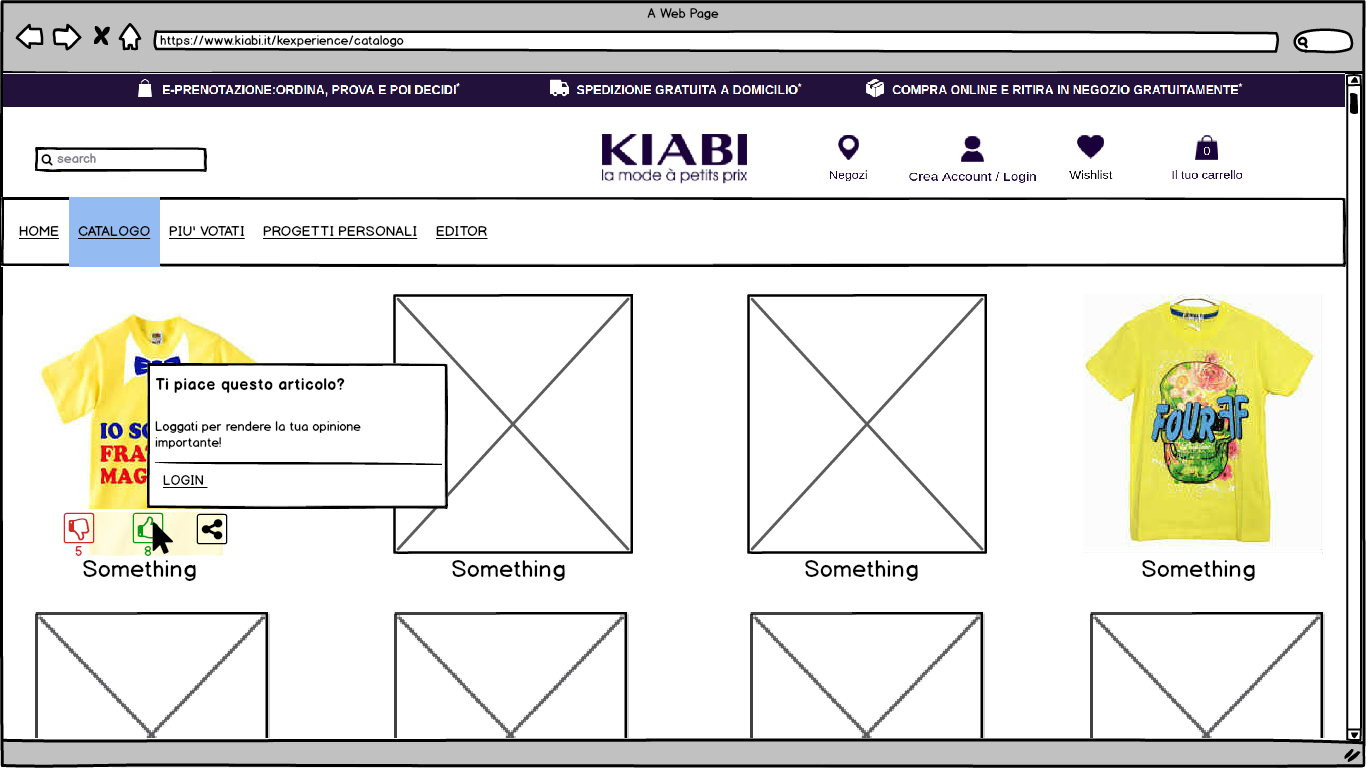
\includegraphics{../../balsamiq/balsamiq_finale/Catalogologin.png}
\caption{Sezione Catalogo - Utente non loggato}
\label{catalogo_non_loggato}
\end{figure}
\clearpage

\newpage
\subsection{Progetti Personali} 

La sezione progetti personali contiene la lista dei prodotti personalizzati dall'utente. Tale sezione è accessible solo dopo che un utente ha effettuato il login.

Come nella sezione catalogo, anche in questo caso è possibile accedere ai dettagli del prodotto con un click sul prodotto stesso.

Facendo over viene data la possiblità di votare (like/dislike), condividere ed eliminare un prodotto. In quest'ultimo caso viene mostrato un modale all'utente per rendere l'operazione più macchinosa in quanto irreversibile.

\begin{figure}[h]
\centering
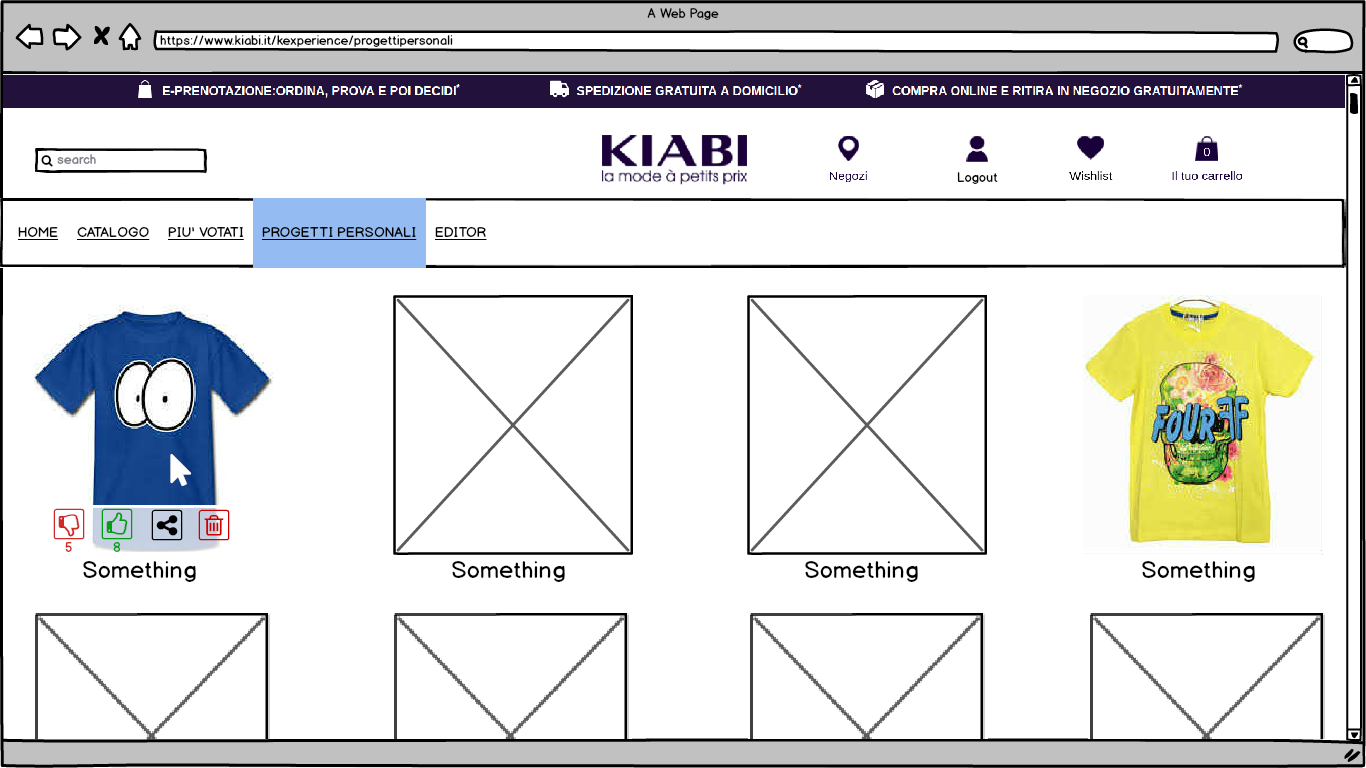
\includegraphics{../../balsamiq/balsamiq_finale/ProgettiPersonali.png}
\caption{Progetti Personali}
\label{progetti_personali}
\end{figure}


\begin{figure}[h]
\centering
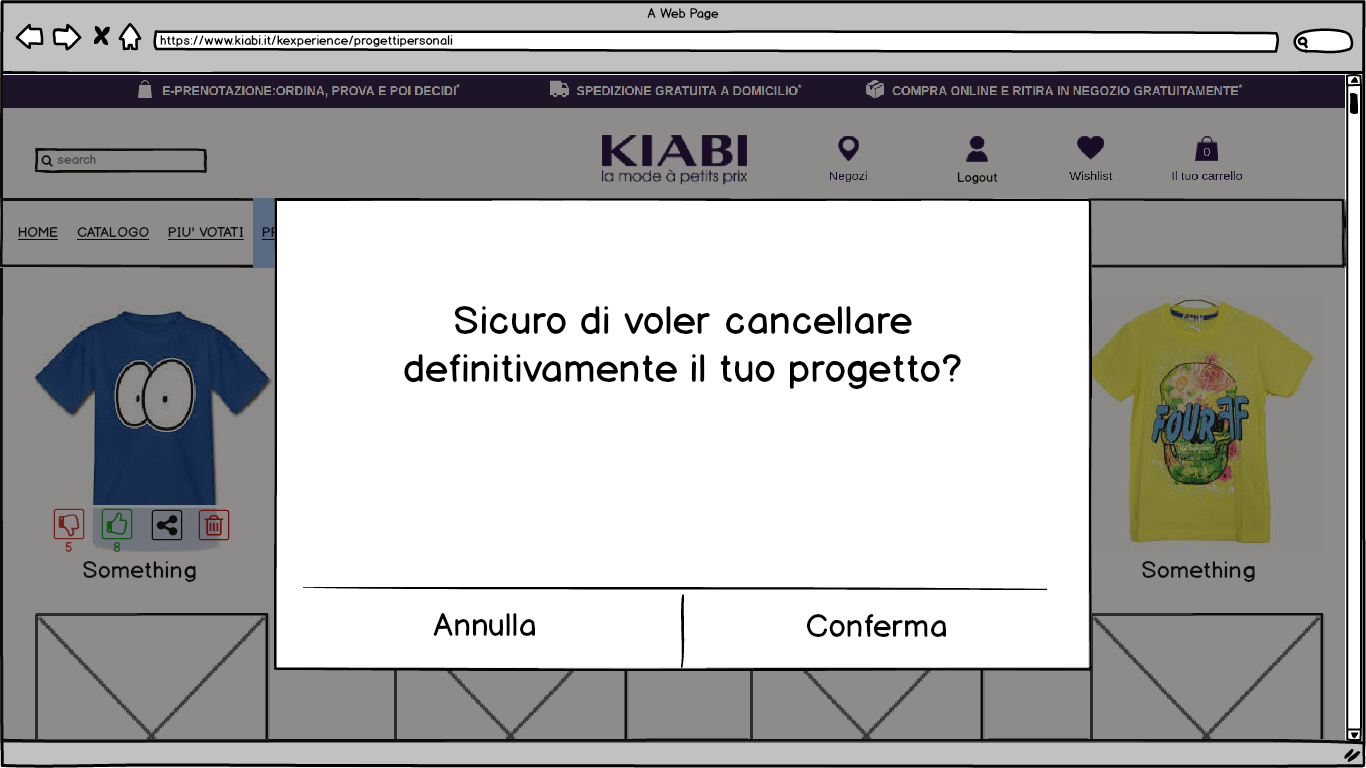
\includegraphics{../../balsamiq/balsamiq_finale/ProgettiPersonalieliminazione.png}
\caption{Progetti Personali - Modale di eliminaizone}
\label{progetti_personali_delete}
\end{figure}
\clearpage


\newpage
\subsection{Progetti più votati} 

La pagina mostra un elenco dei progetti ordinati per differeza tra like/dislike in modo discendente. Per ognuno di essi è presente il nome del progetto, il nome dell'autore, la data di creazione e il numero di like e dislike.

È inoltre presente un bottone "Personalizza" che permette di caricare il progetto scelto direttamente nell'editor per continuare le personalizzazioni (Fig. \ref{piu_votati}).


\begin{figure}[h]
\centering
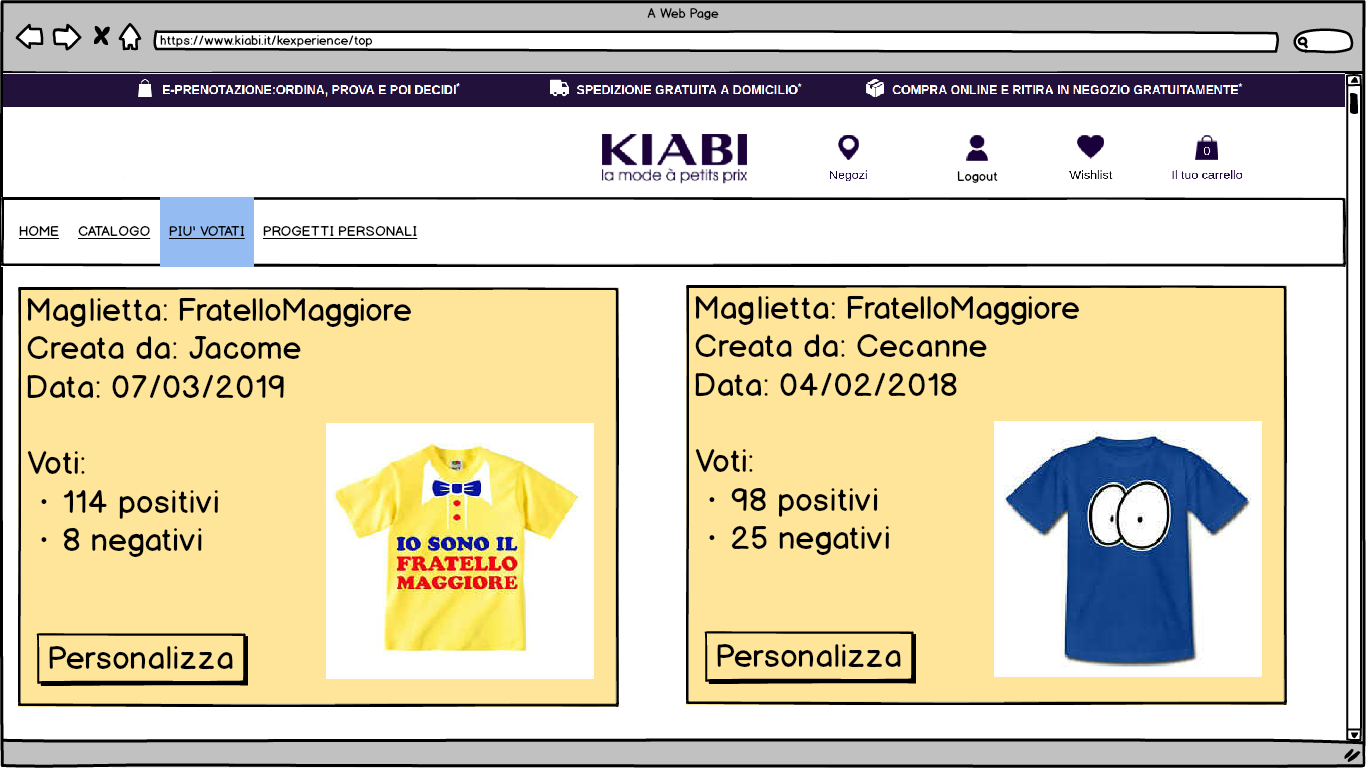
\includegraphics{../../balsamiq/balsamiq_finale/MostRated.png}
\caption{Più Votati}
\label{piu_votati}
\end{figure}


\newpage
\subsection{Editor} 

L'editor è la componente fondamentale di Kids Experience, in quanto permette la vera e propria personalizzazione.

Nella schermata principale dell'editor, sulla parte sinistra, sono presenti quattro miniature che descrivono le macrocategorie personlizzabili: colletto, busto, maniche e taglia. All'interno di ognuna di queste categorie è presente un menù a schede che contiene tutte le possibili personalizzazioni per quella specifica area della maglietta (Fig. \ref{editor}).

Nella barra posta in basso, presente in tutte le varie pagine  dell'editor, sono presenti i link rapidi che permettono di acquistare un prodotto (aggiungendolo al carrello) o di salvarlo nei progetti personali (Fig. \ref{editor_salva}). Inoltre ospita un drop-up menu con la lista delle modifiche (Fig. \ref{editor_listamod}) selezionate e il costo totale aggiornato in tempo reale rispetto modifiche aggiunte.


\begin{figure}[h]
\centering
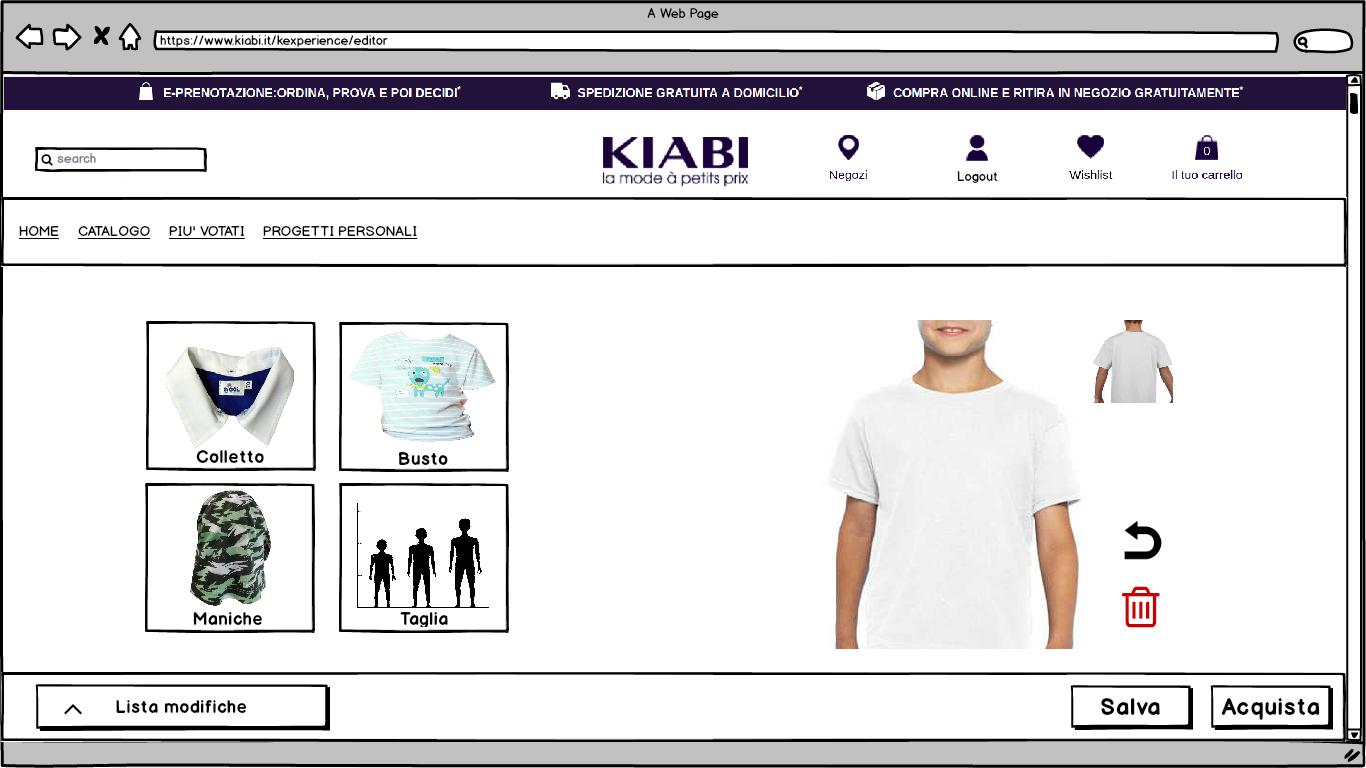
\includegraphics{../../balsamiq/balsamiq_finale/Editorbase.png}
\caption{Editor}
\label{editor}
\end{figure}


\newpage
\subsubsection{Editor Colletto} 

La pagina dell'editor relativa al colletto (Fig. \ref{editor_colletto}) presenta un menù a schede in cui sono presenti tutte le possibili personalizzazioni. In particolare, il tipo di tessuto specifico per quell'area, il tipo di scollo, il colore e i bottoni.

Nella barra posta in basso nella pagina, oltre ai vari link sopracitati, è presente anche il costo totale aggiornato in tempo reale rispetto alle modifiche aggiunte.

\begin{figure}[h]
\centering
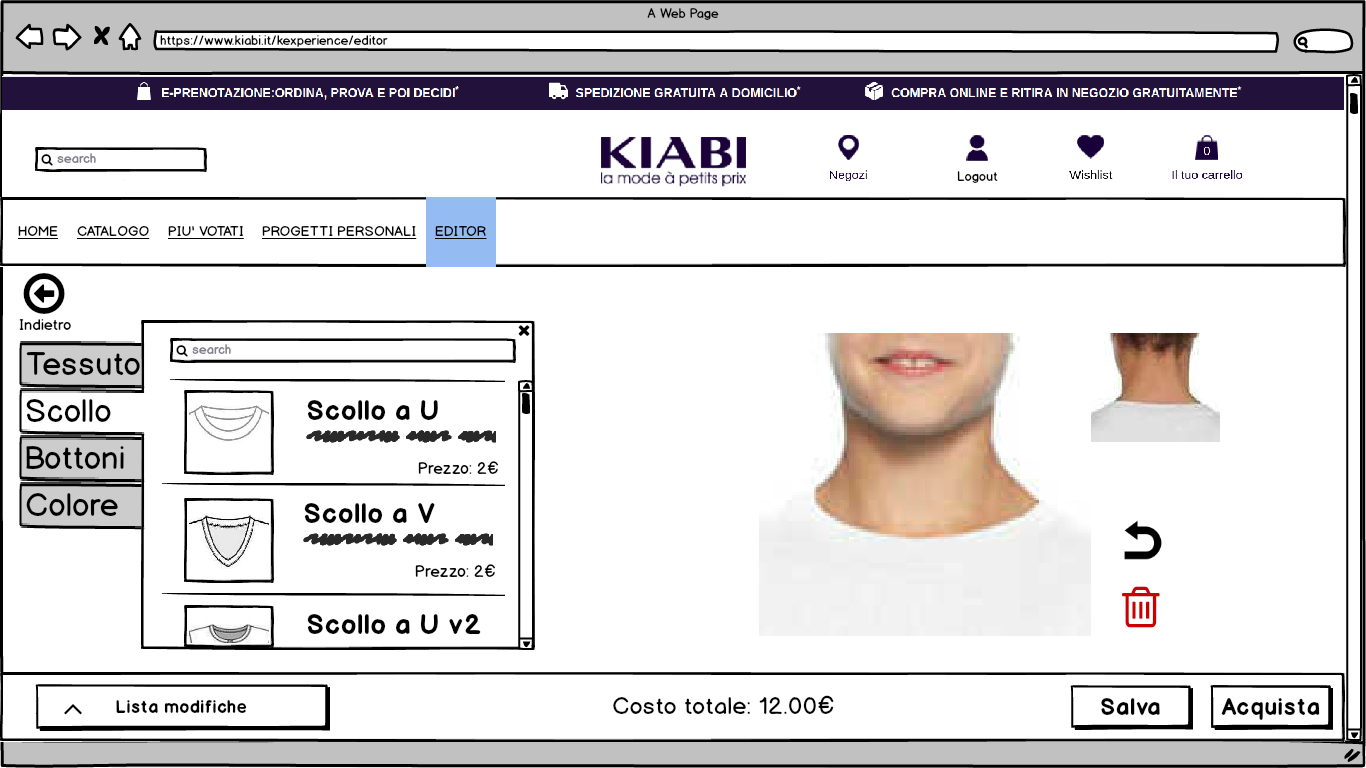
\includegraphics{../../balsamiq/balsamiq_finale/Editor-caratteristicacolloscollo.png}
\caption{Editor - colletto}
\label{editor_colletto}
\end{figure}


\newpage
\subsubsection{Editor Busto} 

La pagina dell'editor relativa al busto (Fig. \ref{editor_busto}) presenta un menù a schede in cui sono presenti tutte le possibili personalizzazioni. In particolare, il tipo di tessuto specifico per quell'area, la possibilità di aggiungere del testo o un'immagine ed il colore.

Nella barra posta in basso nella pagina, oltre ai vari link sopracitati, è presente anche il costo totale aggiornato in tempo reale rispetto alle modifiche aggiunte.

\begin{figure}[h]
\centering
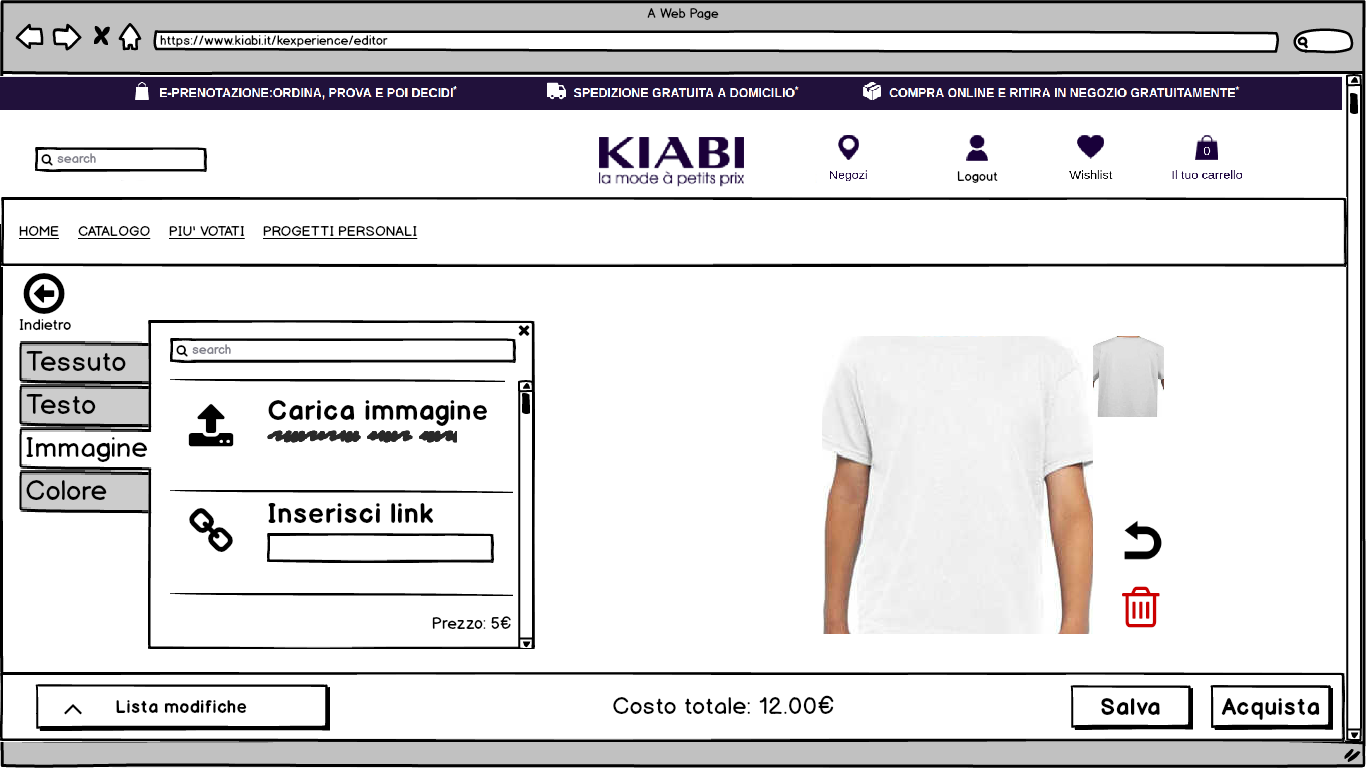
\includegraphics{../../balsamiq/balsamiq_finale/Editor-caratteristicabustoimmagine.png}
\caption{Editor - busto}
\label{editor_busto}
\end{figure}


\newpage
\subsubsection{Editor Maniche} 

La pagina dell'editor relativa alle maniche (Fig. \ref{editor_maniche}) presenta un menù a schede in cui sono presenti tutte le possibili personalizzazioni. In particolare, il tipo di tessuto specifico per quell'area, la possibilità di aggiungere una toppa, una stampa o dei bottoni ed il colore.

Nella barra posta in basso nella pagina, oltre ai vari link sopracitati, è presente anche il costo totale aggiornato in tempo reale rispetto alle modifiche aggiunte.

\begin{figure}[h]
\centering
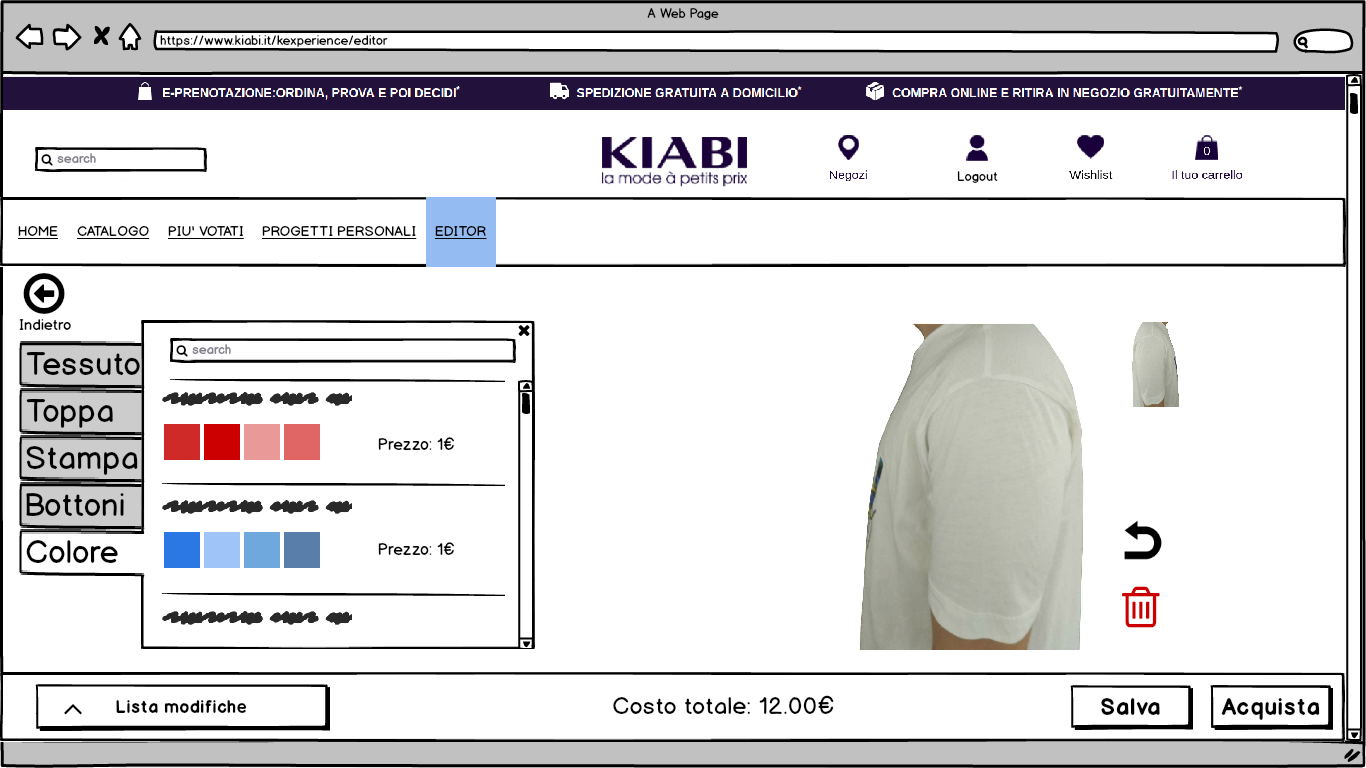
\includegraphics{../../balsamiq/balsamiq_finale/Editor-caratteristicamanichecolore.png}
\caption{Editor - maniche}
\label{editor_maniche}
\end{figure}

\newpage
\subsubsection{Taglia} 

Infine nella pagine dell'editor relativa alla taglia (Fig. \ref{editor_taglia}) è possibile scegliere la misura corretta della maglietta personalizzata o da personalizzare.

Nella barra posta in basso nella pagina, oltre ai vari link sopracitati, è presente anche il costo totale aggiornato in tempo reale rispetto alle modifiche aggiunte.

\begin{figure}[h]
\centering
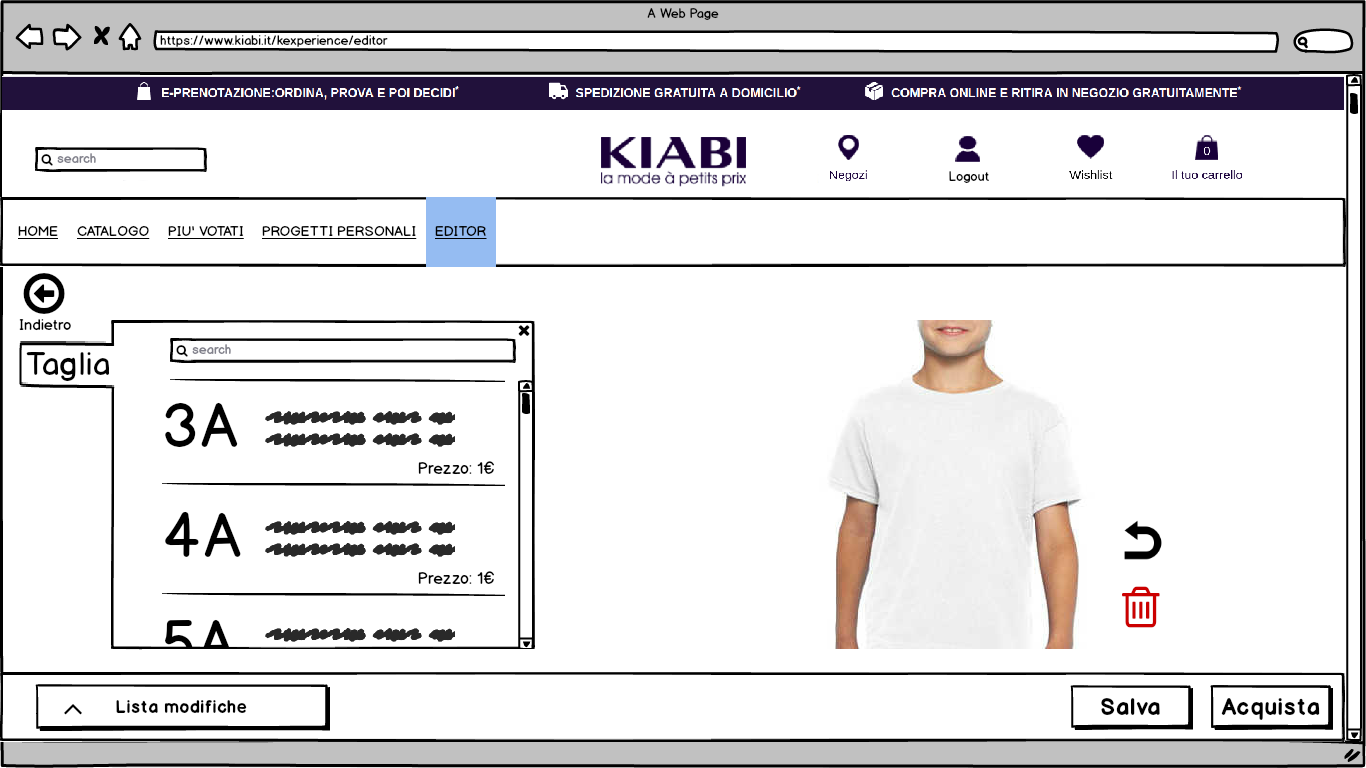
\includegraphics{../../balsamiq/balsamiq_finale/Editor-caratteristicacapotaglia.png}
\caption{Editor - taglia}
\label{editor_taglia}
\end{figure}

\newpage
\subsubsection{Lista Modifiche} 

Ogni volta che viene inserita una personalizzazione, oltre ad essere visualizzata direttamente sul modello, appare anche all'interno della lista delle modifiche, insieme al costo unitario ed un'icona per la rimozione.

\begin{figure}[h]
\centering
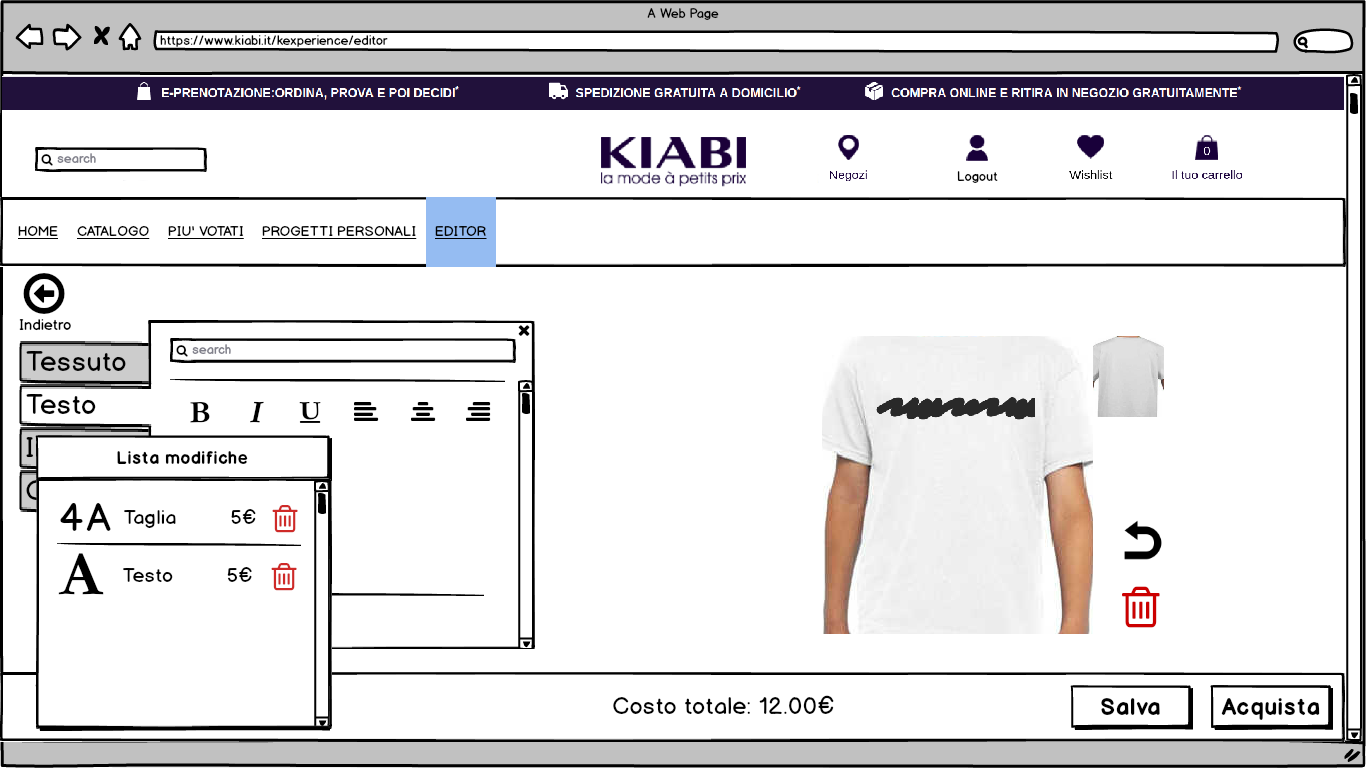
\includegraphics{../../balsamiq/balsamiq_finale/Editor-caratteristicabustotesto4.png}
\caption{Editor - Lista modifiche}
\label{editor_listamod}
\end{figure}


\newpage
\subsubsection{Salvataggio Progetto} 

Come detto precedentemente, in ogni pagina dell'editor è presente un bottone per il salvataggio del proprio progetto (Fig. \ref{editor_salva}). 

Questa funzione è disponibile solo per gli utenti loggati. Se un utente non loggato tentasse di salvare il proprio progetto, si aprirebbe un QUALCOSA in cui è presente un link che rimanda direttamente alla pagina di login (Fig. \ref{login}) e registrazione (Fig. \ref{registrazione}).

\begin{figure}[h]
\centering
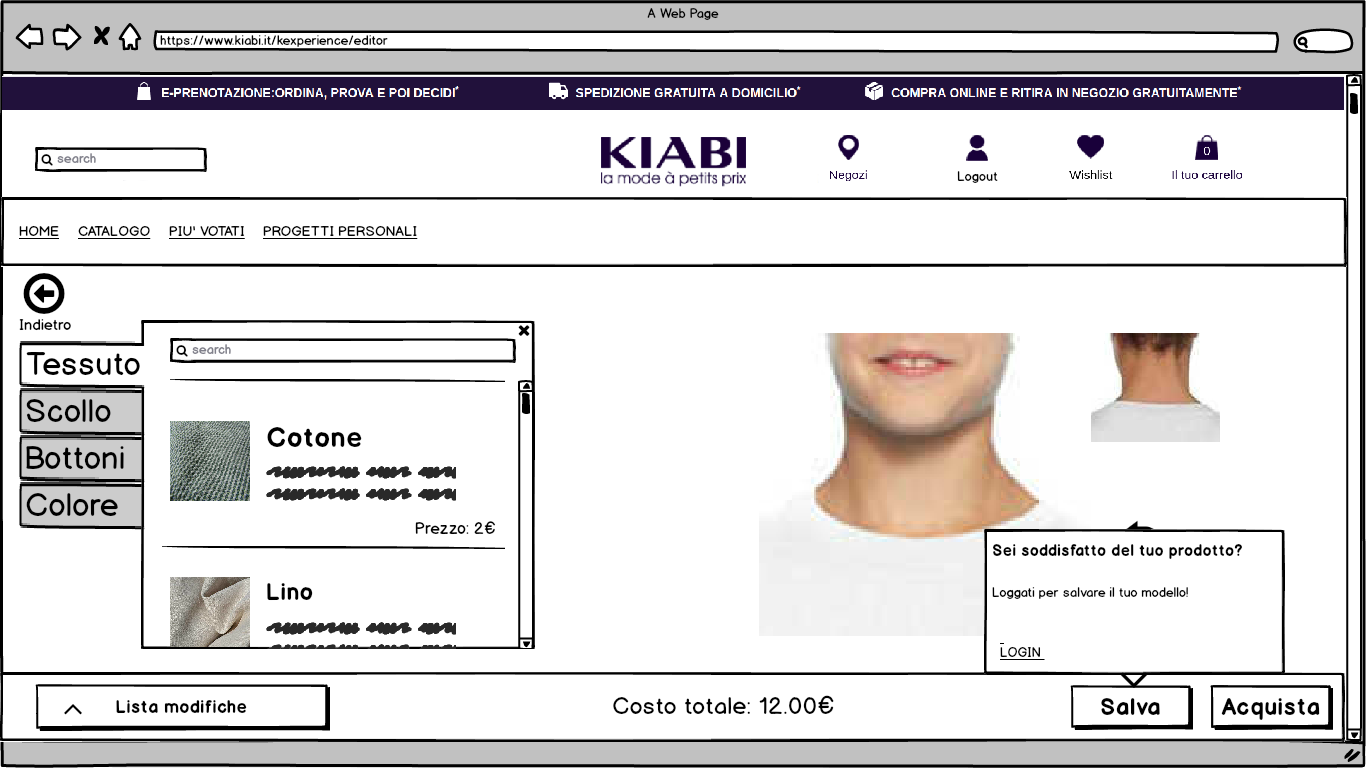
\includegraphics{../../balsamiq/balsamiq_finale/Editor-caratteristicacollotessutononloggato.png}
\caption{Editor - salvataggio progetto}
\label{editor_salva}
\end{figure}


\subsection{Login} 

Il login è una pagina molto semplice che permette l'inserimento delle credenziali di accesso, se l'utente ne è provvisto, altrimenti rimanda alla pagina di registrazione (Fig. \ref{registrazione}).

\begin{figure}[h]
\centering
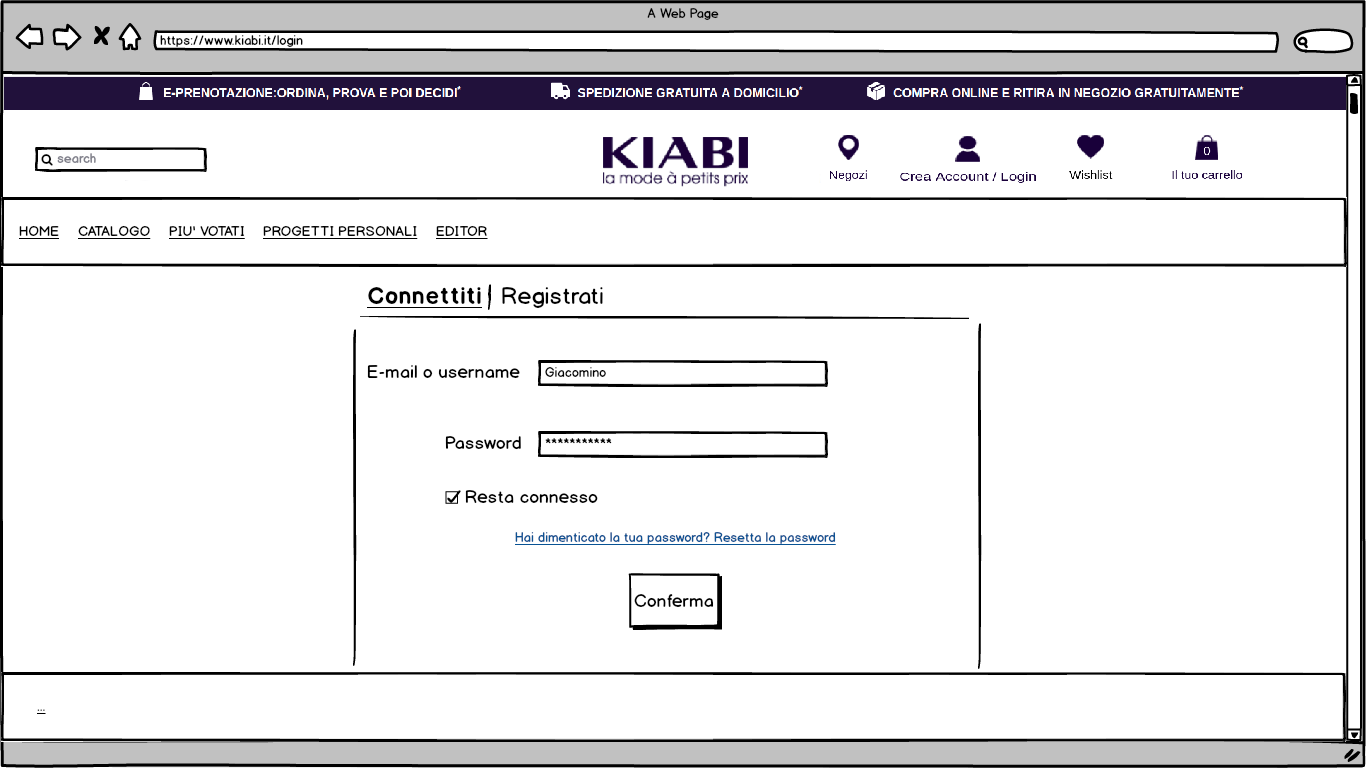
\includegraphics{../../balsamiq/balsamiq_finale/Login.png}
\caption{Login}
\label{login}
\end{figure}


\subsection{Registrazione} 

La pagina di registrazione permette la registrazione dell'utente nel sistema. I campi presenti sono tutti obbligatori.

Se l'utente possiede già un account viene rimandato alla pagina di login (Fig. \ref{login}).

\begin{figure}[h]
\centering
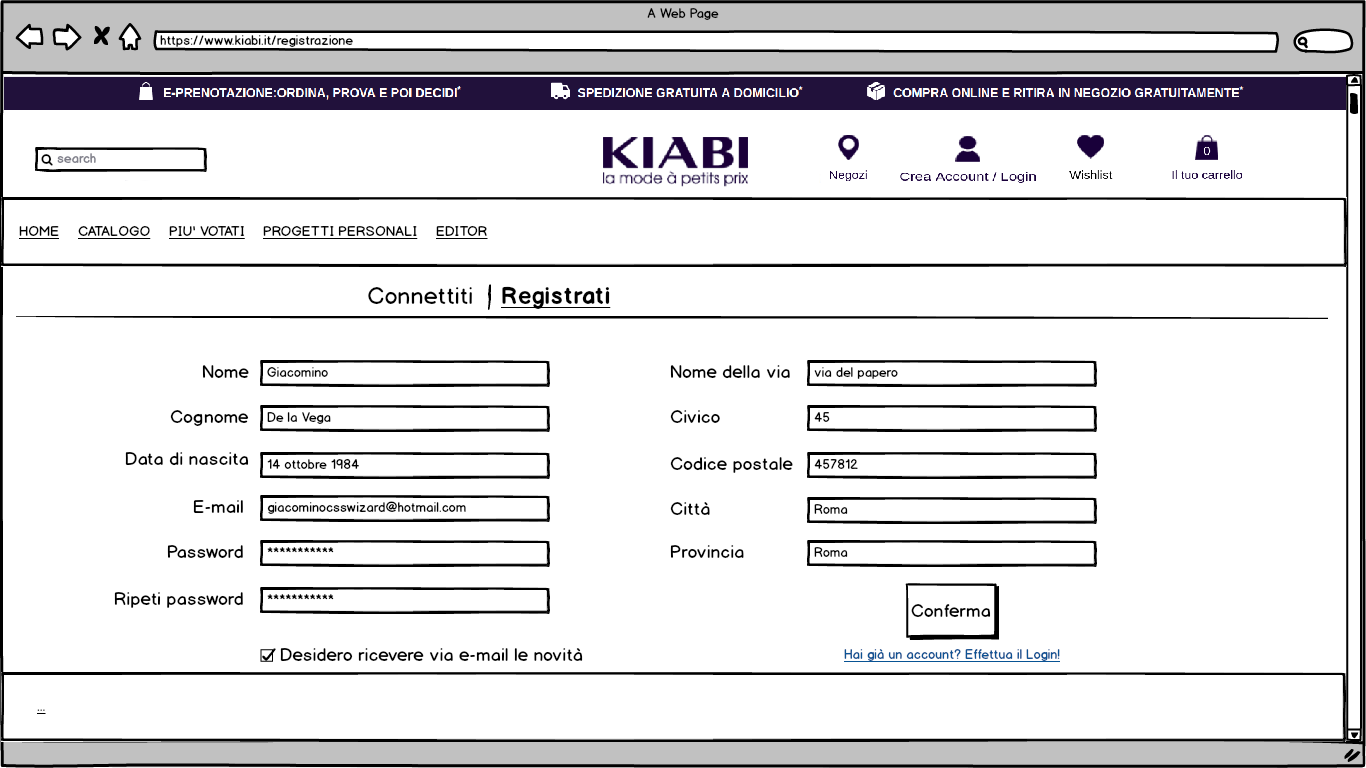
\includegraphics{../../balsamiq/balsamiq_finale/Registrazione.png}
\caption{Registrazione}
\label{registrazione}
\end{figure}
\clearpage 





\newpage
\subsection{Carrello} 

Il carrello (Fig. \ref{carrello}) contiene sia le magliette personalizzate su Kids Experience che i capi d'abbigliamento presenti in Kiabi, che l'utente ha intenzione di acquistare. 

È possibile modificare la quantità di ogni singolo prodotto, eliminare un prodotto dal carrello, controllare il prezzo e procedere all'acquisto.

Inoltre, premendo sui vari capi d'abbigliamento presenti, si apre un modale riepilogativo del prodotto (Fig. \ref{carrello_dett}), che offre la possibilità di caricarlo direttamente nell'editor per proseguire con le modifiche. 


\begin{figure}[h]
\centering
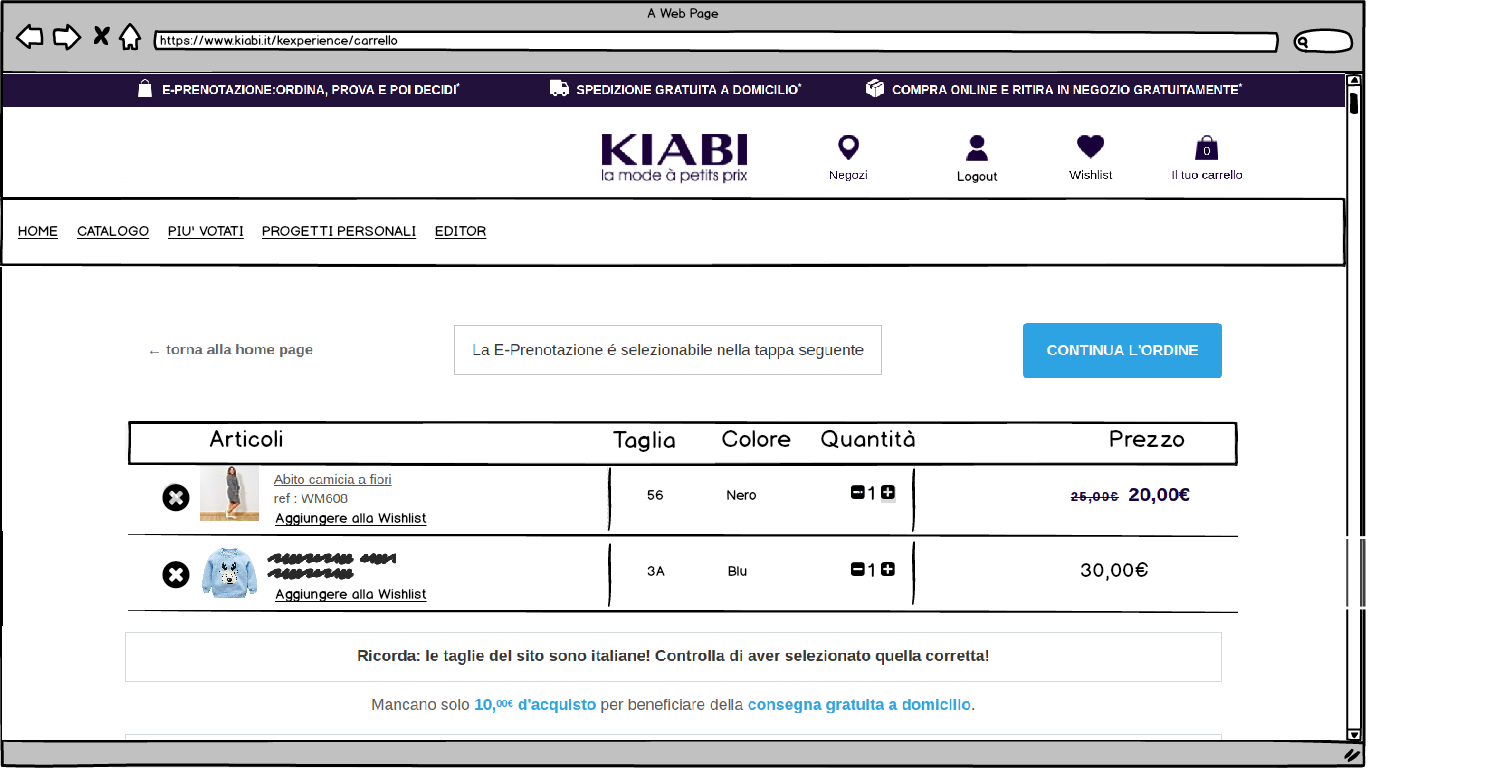
\includegraphics{../../balsamiq/balsamiq_finale/Carrello.png}
\caption{Carrello}
\label{carrello}
\end{figure}

\newpage
\subsubsection{Dettagli Carrello} 

\begin{figure}[h]
\centering
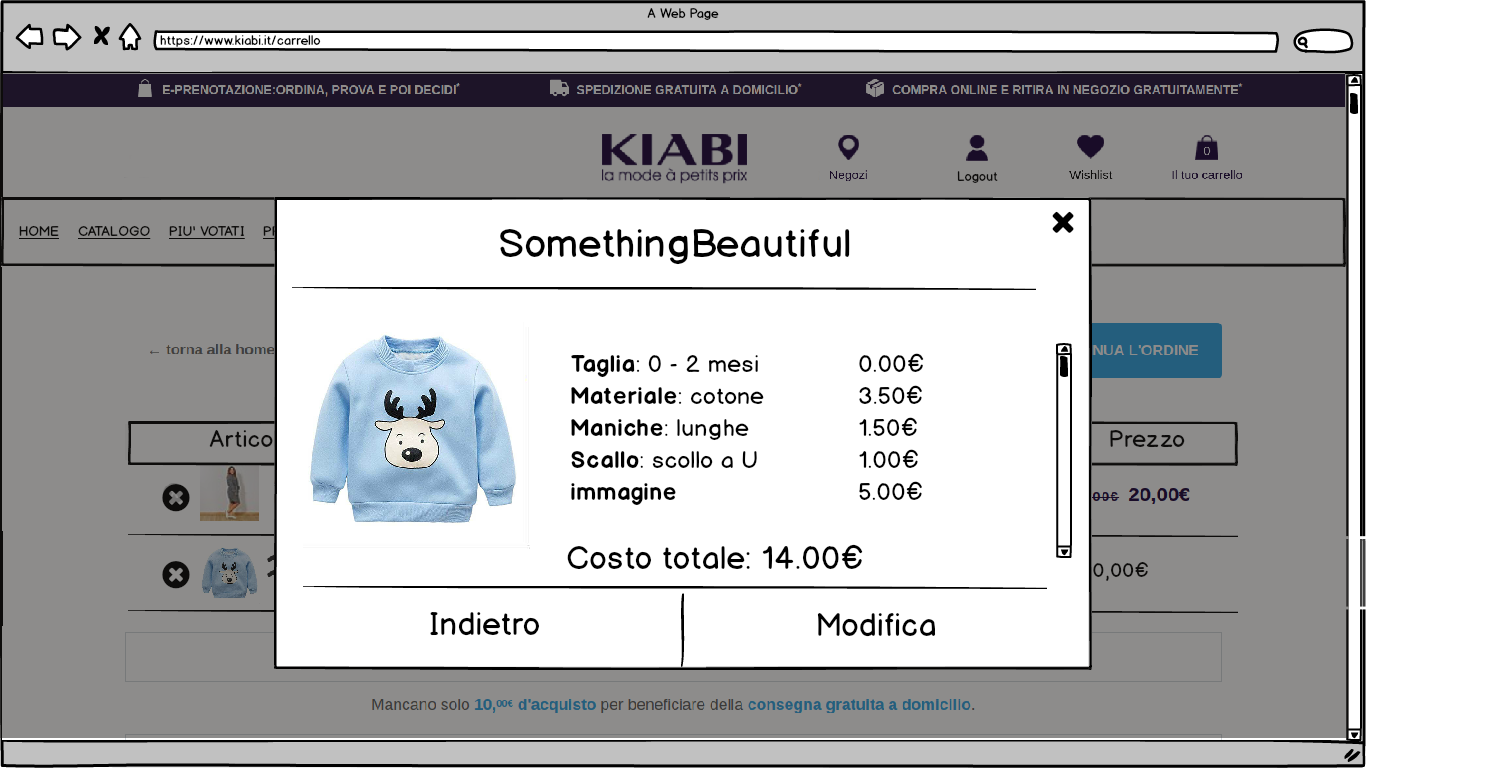
\includegraphics{../../balsamiq/balsamiq_finale/Carrellodettagli.png}
\caption{Carrello - dettagli}
\label{carrello_dett}
\end{figure}


\newpage
\section{Conclusioni}

Kids Experience nasce con l'intento di rilanciare l'attività nel settore dell'abbigliamento per bambini di Kiabi. 
È un'idea innovativa in quanto i negozi della grande distribuzione non sono soliti a creare prodotti personalizzati in base ai gusti dell'utente. 

Il sistema è stato creato da zero, prendendo come riferimento il sito Kiabi.com. 
I test utente effettuati sul sistema esistente hanno permesso di individuare gli errori più comuni, permettendoci di non ripeterli nella realizzazione di Kids Experience.
I successivi test effettuati in modo iterativo su Kids Experience hanno consentito di correggere di volta in volta gli errori ritenuti più gravi.

Visti i risultati ottenuti nei questionari SUS possiamo affermare con certezza che Kids Experience ha un'alta \emph{Learnability}, ovvero un'alta facilità di apprendimento, ed una \emph{Usability} media. Questi risultati sono particolarmente soddisfacenti se consideriamo che il prodotto offerto è una novità per questo tipo di aziende e propone un concetto nuovo come l'estrema personalizzazione di magliette.

Per quanto riguarda gli sviluppi futuri, si prevede un buon margine di miglioramento andando sia ad ampliare le categorie di prodotti personalizzabili sia aumentando il numero di personalizzazioni disponibili.

\newpage
\section{Licenza}\label{licenza}


\includegraphics{img/licenza.png}

Quest'opera è rilasciata sotto una licenza
\href{https://creativecommons.org/licenses/by-nc-sa/4.0/}{Creative
Commons Attribution-NonCommercial-ShareAlike 4.0 International License}.


\end{document}

